\documentclass[]{tufte-handout}

% ams
\usepackage{amssymb,amsmath}

\usepackage{ifxetex,ifluatex}
\usepackage{fixltx2e} % provides \textsubscript
\ifnum 0\ifxetex 1\fi\ifluatex 1\fi=0 % if pdftex
  \usepackage[T1]{fontenc}
  \usepackage[utf8]{inputenc}
\else % if luatex or xelatex
  \makeatletter
  \@ifpackageloaded{fontspec}{}{\usepackage{fontspec}}
  \makeatother
  \defaultfontfeatures{Ligatures=TeX,Scale=MatchLowercase}
  \makeatletter
  \@ifpackageloaded{soul}{
     \renewcommand\allcapsspacing[1]{{\addfontfeature{LetterSpace=15}#1}}
     \renewcommand\smallcapsspacing[1]{{\addfontfeature{LetterSpace=10}#1}}
   }{}
  \makeatother

\fi

% graphix
\usepackage{graphicx}
\setkeys{Gin}{width=\linewidth,totalheight=\textheight,keepaspectratio}

% booktabs
\usepackage{booktabs}

% url
\usepackage{url}

% hyperref
\usepackage{hyperref}

% units.
\usepackage{units}


\setcounter{secnumdepth}{-1}

% citations

% pandoc syntax highlighting

% longtable

% multiplecol
\usepackage{multicol}

% strikeout
\usepackage[normalem]{ulem}

% morefloats
\usepackage{morefloats}


% tightlist macro required by pandoc >= 1.14
\providecommand{\tightlist}{%
  \setlength{\itemsep}{0pt}\setlength{\parskip}{0pt}}

% title / author / date
\title{Biomarker Sample Summary}
\author{Ross Whippo}
\date{10/17/2019}

\usepackage{booktabs}
\usepackage{longtable}
\usepackage{array}
\usepackage{multirow}
\usepackage{wrapfig}
\usepackage{float}
\usepackage{colortbl}
\usepackage{pdflscape}
\usepackage{tabu}
\usepackage{threeparttable}
\usepackage{threeparttablex}
\usepackage[normalem]{ulem}
\usepackage{makecell}
\usepackage{xcolor}

\begin{document}

\maketitle




\hypertarget{overview-of-samples-collected}{%
\subsection{Overview of samples
collected}\label{overview-of-samples-collected}}

\newthought{Over the course} of the expedition, a total of 1508 unique
samples were collected including members of 13 phyla, 14 classes, 101
genera, and 100
species\footnote{Currently, organisms that are not identified to the species level result in the discrepancy between number of genera and species.}.

\(~\)

\textbf{Phyla}

\begin{verbatim}
##  [1] "Echinodermata" "Mollusca"     
##  [3] "Arthropoda"    "Chordata"     
##  [5] "Annelida"      "Bryozoa"      
##  [7] "Cnidaria"      "Rhodophyta"   
##  [9] "Porifera"      "Ochrophyta"   
## [11] "Brachiopoda"   "Chlorophyta"
\end{verbatim}

\textbf{Classes}

\begin{verbatim}
##  [1] "Asteroidea"      "Gastropoda"     
##  [3] "Echinoidea"      "Malacostraca"   
##  [5] "Anthozoa"        "Florideophyceae"
##  [7] "Demospongiae"    "Phaeophyceae"   
##  [9] "Pycnogonida"     "Holothuroidea"  
## [11] "Polyplacophora"  "Bivalvia"       
## [13] "Ulvophyceae"
\end{verbatim}

A total of 1136 invertebrate and 372 algal samples from 15 different
sites were
collected\footnote{These numbers are approximate due to issues identified above.}.

\(~\)

Number of specimens collected varied by specific site, latitude, and ice
cover.

\begin{marginfigure}
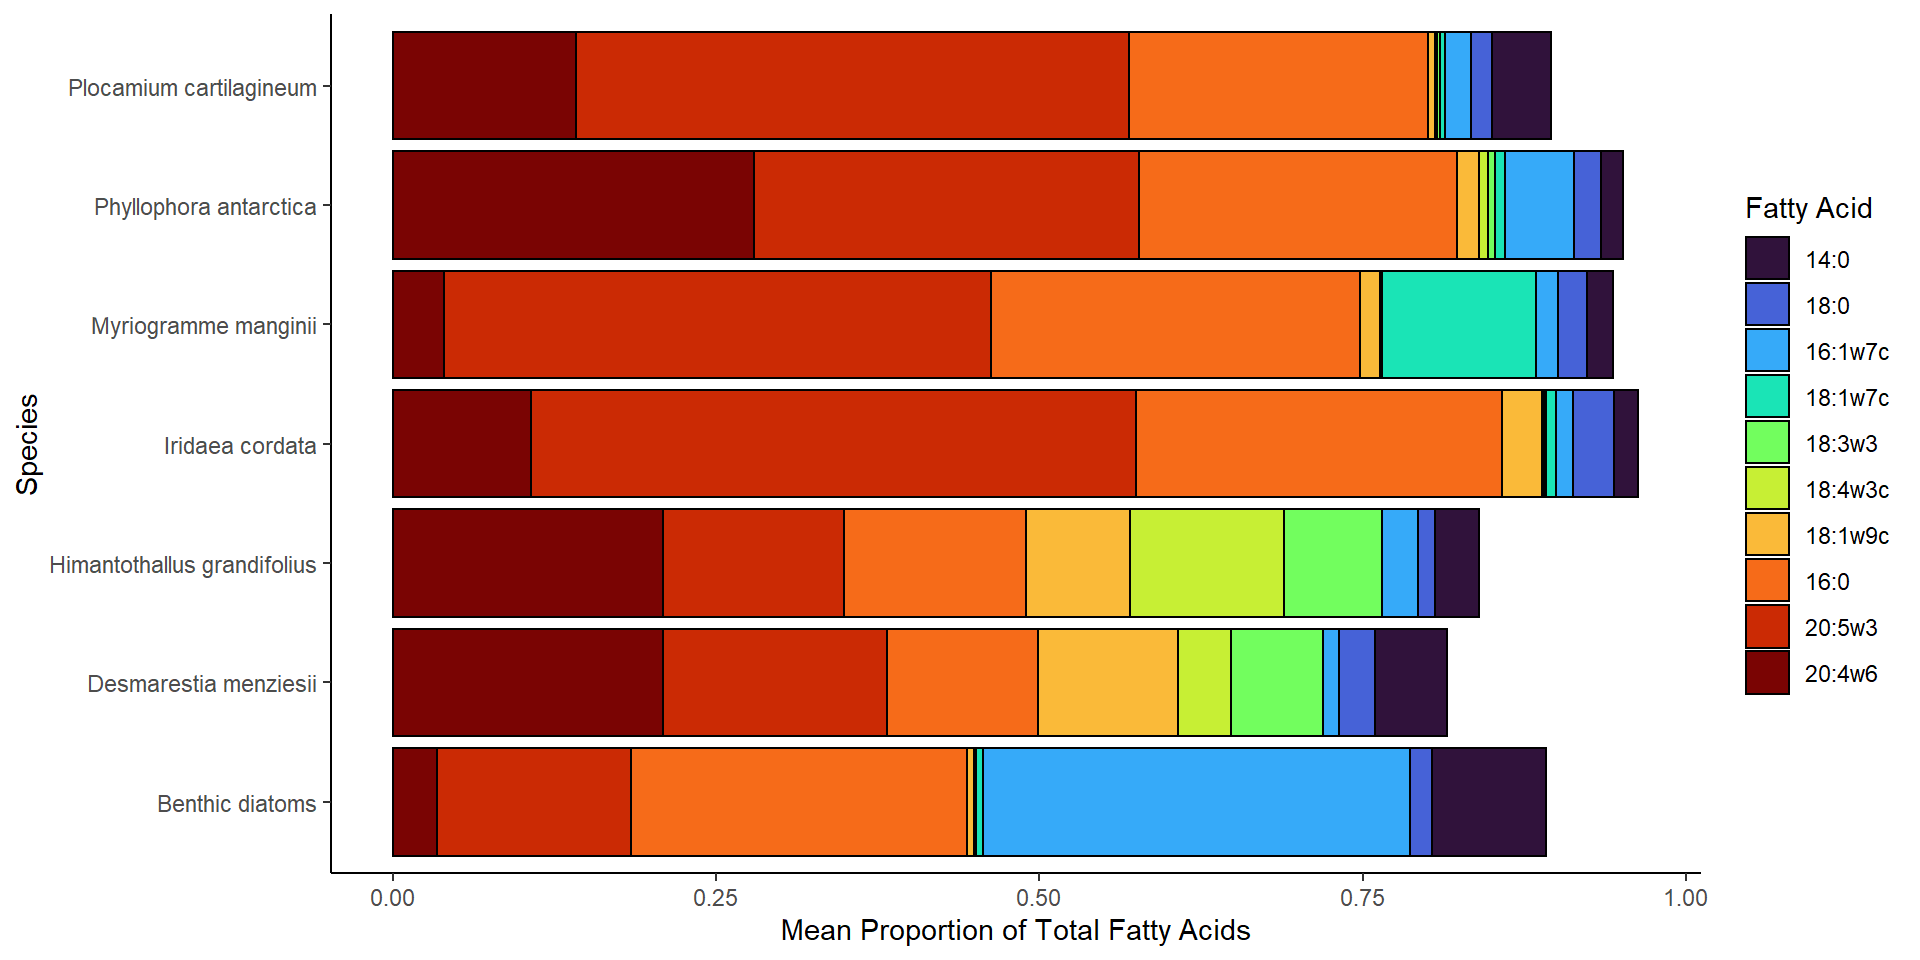
\includegraphics{GradientsBiomarkerSamples_files/figure-latex/unnamed-chunk-5-1} \end{marginfigure}

\begin{marginfigure}
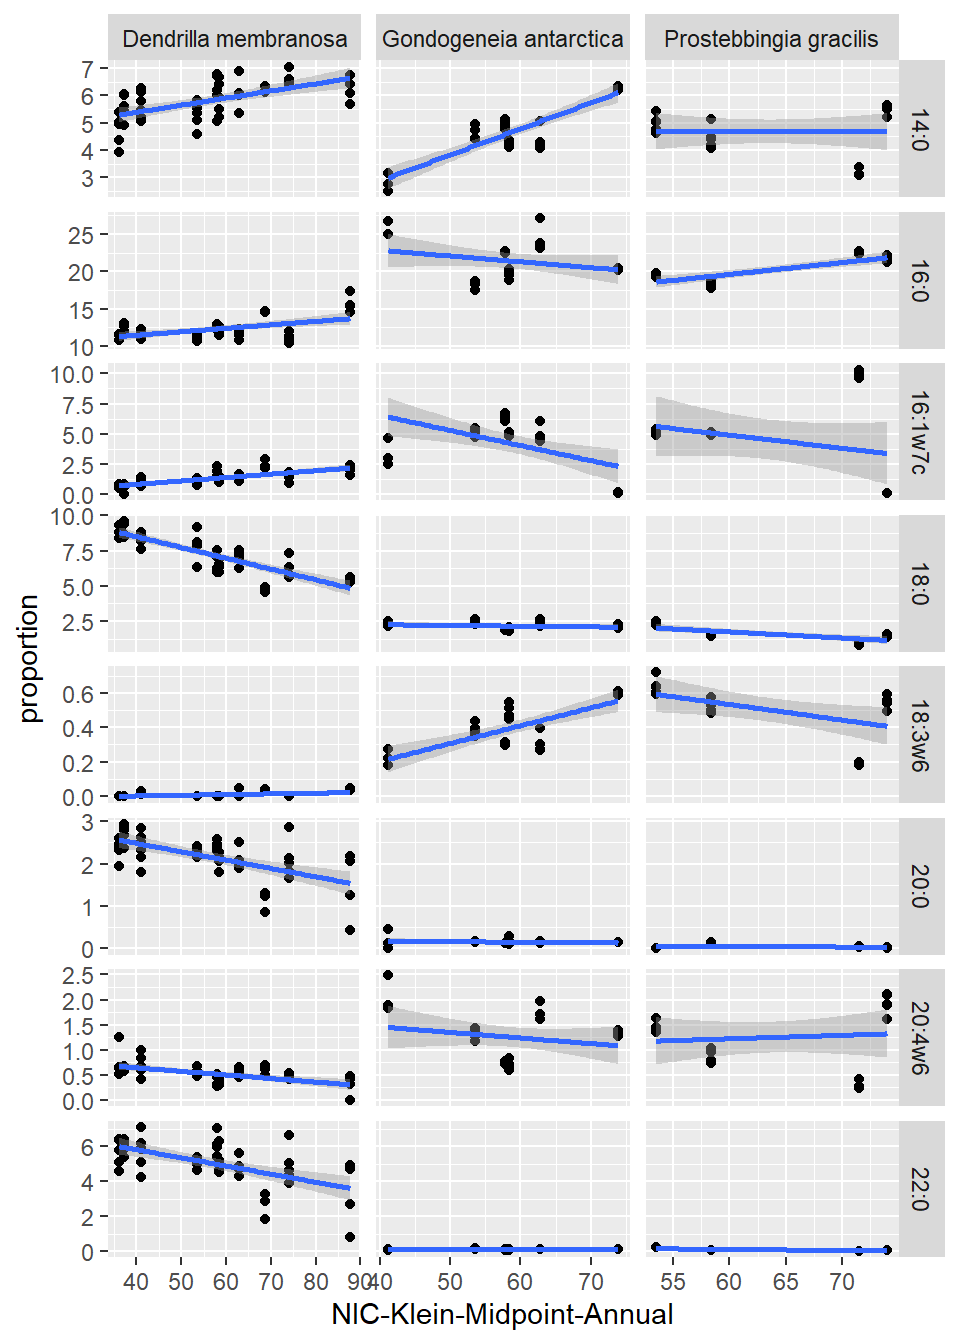
\includegraphics{GradientsBiomarkerSamples_files/figure-latex/unnamed-chunk-6-1} \end{marginfigure}

\hypertarget{summary-of-invertebrates-collected}{%
\subsection{Summary of invertebrates
collected}\label{summary-of-invertebrates-collected}}

\newthought{Number of invertebrates} collected varied by specific site,
latitude, and ice cover parameters. The greatest number of samples were
collected at: sites 05, 07:12, and 14:15 (\textgreater{}100 samples);
ice cover categories 0.4, 0.6, and 0.8 (\textgreater{}300 samples); and
at latitudes to be determined.

Invertebrates present with at least two replicates at all sites include
\emph{Nacella concinna} and \emph{Odontaster validus}.

\begin{table}[H]
\centering
\begin{tabular}{l|r|r}
\hline
value & reps & sites\\
\hline
Bovallia gigantea & 3 & 6\\
\hline
Cnemidocarpa sp. & 3 & 6\\
\hline
Dendrilla membranosa & 3 & 6\\
\hline
Desmarestia menziesii & 3 & 6\\
\hline
Gondogeneia antarctica & 3 & 6\\
\hline
Himantothallus grandifolius & 3 & 6\\
\hline
Iridaea cordata & 3 & 6\\
\hline
Isotealia antarctica & 3 & 6\\
\hline
Margarella antarctica & 3 & 6\\
\hline
Myriogramme manginii & 3 & 6\\
\hline
\end{tabular}
\end{table}

\hypertarget{summary-of-algae-collected}{%
\subsection{Summary of algae
collected}\label{summary-of-algae-collected}}

You can also include things in the margin that are not numbered with the
margin note command\marginnote{Like this.}.

\begin{verbatim}
this is inline code.
\end{verbatim}



\end{document}
